\chapter{The ART Framework}
\label{ch:art}

The ART Framework is a project funded by EIT Digital in collaboration with Politecnico di Milano, Fifthingenium S.r.l.s., Technische Universität Berlin and TIM that aims at creating an Extended Reality as a Service (XRaaS) platform to enhance tourism in places with a high historical, cultural and artistic value. The platform aims to make programming experiences in XR accessible to non-IT experts. By stimulating the spread of XR applications, it is hoped that the tourism sector will also benefit from significant growth. Different stakeholders are involved, as tour operators, event organizers and museum curators, with the mission to create a unique tourist experience, starting from the decision-making process for a destination to the on-site experience, combining artistic locations with virtual tour guides and digital contents.

As we have described in \autoref{sec:background-tourism-xr}, \gls{XR} technologies are finally mature to be widely deployed in the tourism sector, also thanks to the variety of devices coming on the market. Furthermore, the new 5G internet connection will enable high-quality low-latency streaming of contents, higher download speeds, real-time interactions and multi-user experiences.

The ART project will hence provide a service for all the players involved in the tourism industry that allows the creation of \gls{XR} experiences without the need to code and deploy multiple applications but directly supporting the acquisition of digital contents, their processing and final transformation into assets downloadable and playable on different \gls{AR}/\gls{VR} devices where these experiences are rendered.

In this chapter, \autoref{sec:art-overview} will give an overview to the technological stack of ART and the workflow that enables the creation of XR apps; later, \autoref{sec:art-editor} will explain in detail the ART Editor,the application supporting the authoring process of these experiences,  inspired by the conceptual model introduced in \autoref{ch:conceptual-model}.

\section{System Overview}
\label{sec:art-overview}

The system architecture of the ART XRaaS is composed by different modules, each reflecting a phase of the creation process of an \gls{XR} experience (\autoref{fig:architecture}). The system is composed as follows:
\begin{itemize}
    \item A \textbf{Content Management System} (CMS) implements the \emph{assets upload phase}. It is a web application acting as entry point into the creation process, where designers of the \gls{XR} experience create or open an existing project and upload all the digital contents to be included in the next phases. It is served by a database to persist and retrieve assets, which can be 3D models (\textit{.fbx, .obj}), images or textures (\textit{.jpeg, .bmp, .png}), video clips (\textit{.mp4}), audio tracks (\textit{.mp3}), text documents (\textit{.txt}), QR Codes (described by their plain text content) and object-related operational entities (a \textit{menu}). Lastly, the application allows to categorize and label these assets, assigning them to different \emph{Scenes}.

    \item The \textbf{ART Editor} is involved in the \emph{interaction authoring phase}. It is a web application that, after retrieving all the assets already uploaded in the previous phase, allows to model in a canvas the interactions among these entities according to user inputs, using a "state-action-effect" paradigm typical of Finite State Machines (FSM). Indeed, the experience is described by a sequence of States connected by Actions, where each State contains different objects and each object has specific properties that can change. After modeling the interactions, the Editor allows to save the flow of the experience in a configuration file used in the next phase.
    
    \item A \textbf{\gls{HMD} Authoring Application} allows the \emph{on-site authoring phase}: during this phase the user, wearing a \gls{HMD}, opens the created project and a \emph{run-time engine} parses the configuration file exported in the previous phase; then, the application downloads all the assets from the CMS' database to proceed in the authoring process. During this phase the authors of the experience set each Scene, placing the assets in the virtual environment and configuring their properties such as position, scale and orientation; in the case of \gls{AR} authoring they map the coordinates of the physical environment with the digital one through \emph{Spacial Anchors}\footnote{\url{https://azure.microsoft.com/en-us/services/spatial-anchors/}} to persist the coordinates of digital contents with respect to real environment. 
    
    \item The on-site authoring phase is the last phase of the development process and, for complimentary, here we cite the last component of the system, that is the \textbf{Universal \gls{XR} Application Reader}. This is the final application for the end user (the tourist) that consists in a run-time engine responsible for the correct parse of the configuration file and rendering of the virtual environment. This application is available for both \glspl{HHD} and \glspl{HMD}, and in the latter case both for \gls{AR} and \gls{VR} devices.
\end{itemize}

\begin{figure}[h]
    \centering
    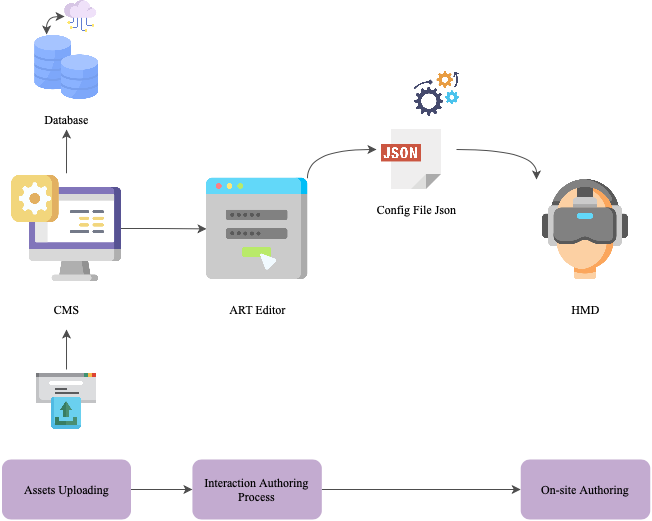
\includegraphics[width=\textwidth]{Figures/Editor/architecture.png}
    \caption{System Overview - Architecture}
    \label{fig:architecture}
\end{figure}

\subsection{ART User Journey}
\label{subsec:art-user-journey}

To give the reader a better understanding of the way the system works we provide a user journey considering the example of a cultural heritage site whose curators are interested in enhancing the experience of their visitors through \gls{XR} technologies. Their goals is to augment the information of the exhibits through virtual panels containing descriptions, historical videos, pictures and reconstruction models of the past; using the ART Framework it is only required some expertise in 3D content authoring to create the models, while the app development part is totally transparent to the user thanks to ART XRaaS. The user journey to develop the \gls{XR} experience would be the following:
\begin{enumerate}
    \item The user produces 3D models and gathers all the digital and multimedia assets contributing to the experience.
    \item The user accesses the web portal of the ART CMS and create a new project.
    \item The user upload all the assets on the CMS, then they define their properties such as names and labels to support the next development phase and, if necessary, cluster each of them in different scenes.
    \item The user opens the ART Editor and define the end user (tourist) interactions with the elements through a canvas and a "state – action – effect" paradigm.
    \item The user save the modelled experience and a configuration file is exported.
    \item The user, wearing a Microsoft HoloLens 2 \gls{HMD}, opens the exported configuration file using the on-site authoring application.
    \item The user decide to create an \gls{AR} application and scan the heritage site to place Spatial Anchors in it; to do so, they place the assets in the environment choosing their placement, size and orientation by manipulating these elements through \emph{gestures}.
    \item Finally, they save and publish the app that will be available for tourists, regardless of the \gls{AR} device used to augment their visit.
\end{enumerate}
\section{ART Editor}
\label{sec:art-editor}

\subsection{From the Conceptual Model to the Editor}
\label{subsec:art-editor-from-conceptual}
\clearpage
\subsection{High-Level Design}
\label{subsec:art-editor-highlevel}

The high-level design of the ART Editor started from an analysis of goals and requirements in projecting and developing an XR application, considering the phases of the framework as described in \autoref{sec:art-overview}. Hence, this study was based on how to specify the run-time behaviour of virtual elements presented in \gls{AR}/\gls{VR} scenes. The goals of the \gls{XR} editor as a component of the ART Framework are:
\begin{itemize}
    \item[\textbf{G1}] The editor supports the design of AR and VR experiences
    \item[\textbf{G2}] The editor allows to model the interactions between users and virtual objects in a scene and the corresponding behaviour of the last ones
    \item[\textbf{G3}] The editor allows to model the interactions and behaviours on elements already uploaded on a Content Management System
    \item[\textbf{G4}] The editor is part of a workflow in the creation of XR experiences and allows to export a modelled environment, as well as load it
    \item[\textbf{G5}] The editor can describe the properties of the elements it supports and their changes
    \item[\textbf{G6}] The editor is based on a syntactically and semantically valid conceptual model
    \item[\textbf{G7}] The editor works on a web application for desktop browsers
\end{itemize}

After having understood which capabilities the XR editor needed to achieve, we started defining the functional requirements to meet during the development of the tool:
\begin{itemize}
    \item[\textbf{R1}] The editor is based on the XRM Conceptual Model
    \item[\textbf{R2}] The editor represents user actions directly on the target elements
    \item[\textbf{R3}] The editor represents elements' run-time properties in 'states' of the application
    \item[\textbf{R4}] The editor allows a flow representation of the interactions
    \item[\textbf{R5}] The editor allows forking and merging of paths in the flow representation for conditional or logic modelling (e.g. logic AND, OR of interactions)
    \item[\textbf{R6}] The editor produces a schema of the modelled experience in order to be read and parsed by the on-site authoring tool
    \item[\textbf{R7}] The editor is able to edit previously modelled experiences
    \item[\textbf{R8}] The editor allows to change the different values of elements only when needed, keeping a clean \gls{UI}
    \item[\textbf{R9}] The editor allows an easy and intuitive UI in order to be used on desktop environments
    \item[\textbf{R10}] The editor allows a technology abstraction modelling
\end{itemize}

\subsubsection*{Editor Specifications}
From the specifications above mentioned and the goals to achieve in order to support the ART Framework in the development of XR applications, we explored the concept (\autoref{fig:art-fsm-sketch}) of an editor representing its elements and their run-time structural properties as a state diagram (\autoref{fig:fsm}) typical of \glspl{FSM}: the behaviour of the application and its virtual objects is described by linked nodes in which user interactions -- corresponding to action nodes -- change the state of these elements, represented in state nodes.
\begin{figure}[h]
    \begin{subfigure}{0.45\columnwidth}
        \centering
        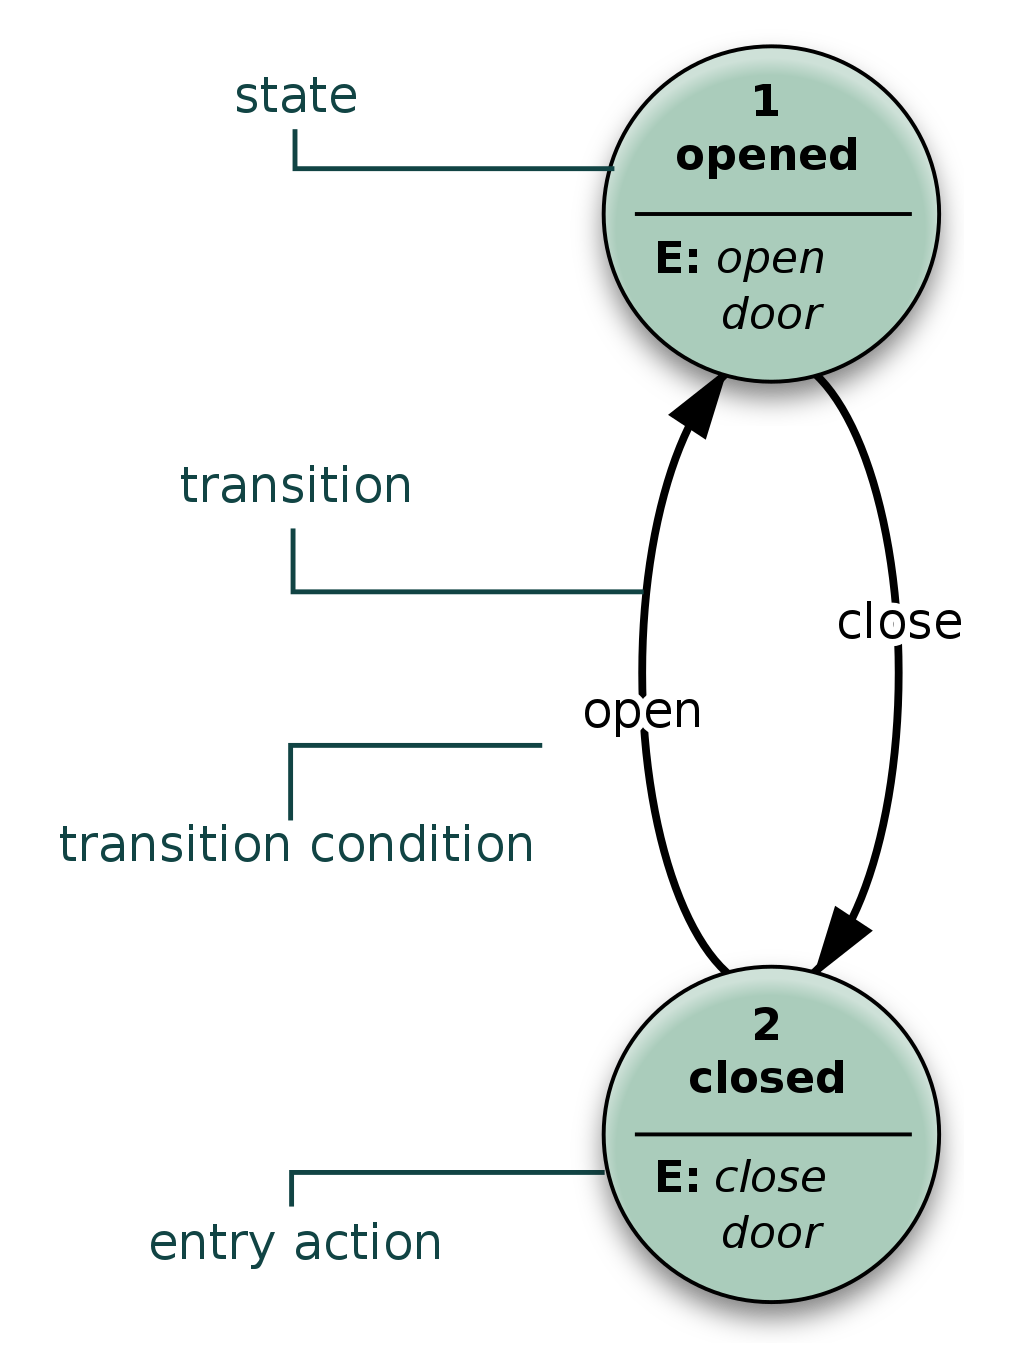
\includegraphics[height=12em]{Figures/Editor/fsm.png}
        \caption{}
        \label{fig:fsm}
    \end{subfigure}
    \begin{subfigure}{0.5\columnwidth}
        \centering
        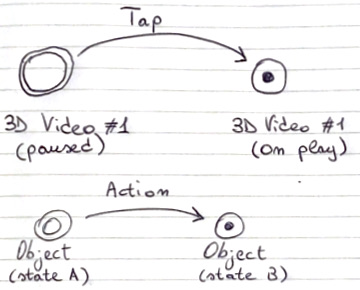
\includegraphics[height=12em]{Figures/Editor/fsm-handwritten.png}
        \caption{}
        \label{fig:art-fsm-sketch}
    \end{subfigure}
    \caption{A door's state diagram (\ref{fig:fsm}) and a handwritten FSM-editor sketch (\ref{fig:art-fsm-sketch})}
\end{figure}

Being a desktop web-application we took full advantage of the web page layout that allows a wider organization of UI components compared to smaller devices (e.g. smartphones); we chose to represent the editor as a blank canvas in which it is possible to draw diagrams representing the XR experience.From the left-hand side panel, all previously loaded assets can be selected as available elements for the editor.
Another feature we thought would allow an easier and cleaner UI is the assignment of actions and properties to elements in the same way -- namely, using a decorator approach to show only relevant property assignments.
Furthermore, the configuration of the modelled experience can be exported, imported and modified using a file describing the diagram, so that it can be supported both by the on-site authoring phase and the interaction authoring phase.

\subsubsection*{Logic Decisions}
The logical high-level design choices consisted of determining the kinds of objects to be modelled in the editor and the actions performed by the user in the interaction. The XRM Conceptual Model in conjunction with the extensive literature review on XR applications in tourism (\autoref{sec:background-tourism-xr}) guided this process, whose first results consisted in choosing the entities (Non-Human Actors) of the XR experience listed in \autoref{table:xrm-art-actors}.

The following step was the definition of the states in which these elements can be distinguished: we decided to cluster the effects on these actors as atomic property modifiers in order to describe as few states as possible for these elements without losing many details in conceptual modelling; for these reasons we found that elements can be in one or more of the following states. \autoref{tab:art-compatible-objects} and \autoref{tab:art-compatible-states} show, respectively, an overview of the available states per entity and the compatibility among different states that can be associated to the same element.

\begin{itemize}
    \item \textbf{Visible} acts on the visibility property -- setting it to 'on' -- and its related opacity
    \item \textbf{Hidden} acts on the visibility property, setting it to 'off'
    \item \textbf{Blinking} enables a luminous border on the target object to attract users' attention
    \item \textbf{Selected} marks the component as selected for more interactions (e.g. manipulation, showing menus, etc.) on it
    \item \textbf{Unselected} deselects the component
    \item \textbf{Manipulated} indicates the component has been manipulated via rotation/translation/scaling
    \item \textbf{On Play} indicates when a multimedia entity is in playback
    \item \textbf{Paused} indicates when a multimedia entity is paused
    \item \textbf{Audio} changes the audio settings, turning it on or off
    \item \textbf{Subtitles} changes the subtitles settings, turning them on or off
\end{itemize}

\begin{table}[h]
\centering
\begin{tabular}{l|c|c|c|c|c|c|c|c|}
\cline{2-9}
 &
  \begin{tabular}[c]{@{}c@{}}3D\\ Scene\end{tabular} &
  \begin{tabular}[c]{@{}c@{}}3D\\ Model\end{tabular} &
  \begin{tabular}[c]{@{}c@{}}3D\\ Video\end{tabular} &
  \begin{tabular}[c]{@{}c@{}}2D\\ Video\end{tabular} &
  \begin{tabular}[c]{@{}c@{}}2D\\ Image\end{tabular} &
  \begin{tabular}[c]{@{}c@{}}2D\\ Text\end{tabular} &
  \begin{tabular}[c]{@{}c@{}}360°\\ Video\end{tabular} &
  Menu \\ \hline
\multicolumn{1}{|l|}{Visible}     & x & x & x & x & x & x & x & x \\ \hline
\multicolumn{1}{|l|}{Hidden}      & x & x & x & x & x & x & x & x \\ \hline
\multicolumn{1}{|l|}{Blinking}    &   & x & x & x & x & x &   & x \\ \hline
\multicolumn{1}{|l|}{Selected}    &   & x & x & x & x & x &   & x \\ \hline
\multicolumn{1}{|l|}{Unselected}  &   & x & x & x & x & x &   & x \\ \hline
\multicolumn{1}{|l|}{Manipulated} &   & x &   &   &   &   &   &   \\ \hline
\multicolumn{1}{|l|}{On Play}     &   &   & x & x &   &   &   &   \\ \hline
\multicolumn{1}{|l|}{Paused}      &   &   & x & x &   &   &   &   \\ \hline
\multicolumn{1}{|l|}{Audio}       &   &   & x & x &   &   & x &   \\ \hline
\multicolumn{1}{|l|}{Subtitles}   &   &   & x & x &   &   & x &   \\ \hline
\end{tabular}
\caption{Compatible objects with states}
\label{tab:art-compatible-objects}
\end{table}

\begin{table}[h]
    \centering
    \begin{tabular}{l|c|c|c|c|c|}
    \cline{2-6}
     & \multicolumn{1}{l|}{Visible} & \multicolumn{1}{l|}{Hidden} & \multicolumn{1}{l|}{Blinking} & \multicolumn{1}{l|}{Selected} & \multicolumn{1}{l|}{Unselected} \\ \hline
    \multicolumn{1}{|l|}{Visible}     &   & X & \checkmark & \checkmark & \checkmark \\ \hline
    \multicolumn{1}{|l|}{Hidden}      & X &   & X & X & \checkmark \\ \hline
    \multicolumn{1}{|l|}{Blinking}    & \checkmark & X &   & \checkmark & \checkmark \\ \hline
    \multicolumn{1}{|l|}{Selected}    & \checkmark & X & \checkmark &   & X \\ \hline
    \multicolumn{1}{|l|}{Unselected}  & \checkmark & \checkmark & \checkmark & X &   \\ \hline
    \multicolumn{1}{|l|}{Manipulated} & \checkmark & X & \checkmark & \checkmark & X \\ \hline
    \multicolumn{1}{|l|}{On Play}     & \checkmark & X & \checkmark & \checkmark & \checkmark \\ \hline
    \multicolumn{1}{|l|}{Paused}      & \checkmark & \checkmark & \checkmark & \checkmark & \checkmark \\ \hline
    \multicolumn{1}{|l|}{Audio}       & \checkmark & X & \checkmark & \checkmark & \checkmark \\ \hline
    \multicolumn{1}{|l|}{Subtitles}   & \checkmark & X & \checkmark & \checkmark & \checkmark \\ \hline
    \end{tabular}
    \caption{Compatibility among states}
    \label{tab:art-compatible-states}
\end{table}

The interactions, required to model virtual objects' changes of states, have been identified following the same process carried out for object states and inspired by XRM Behavioural Model's User Actions (\autoref{tab:BMUserActions}); starting from the table mentioned above, we chose some User Actions and adapted them to the editor and the entire ART Framework, defining their meaning and the objects on which these actions can be performed (\autoref{tab:art-compatible-actions}):
\begin{itemize}
    \item \textbf{Object Recognition} refers to the recognition of QR Codes by the application
    \item \textbf{Voice Command Recognition} is a specific feature for accessibility purposes (e.g. play a content by voice instead of tapping it)
    \item \textbf{Gesture Recognition} enables the modelling of complex gestures defined during the on-site authoring phase
    \item \textbf{Speech to Text} is the action of dictating a text input to the device
    \item \textbf{Proximity In} is the implicit action by a user approaching a virtual content or 3D Scene area
    \item \textbf{Proximity Out} is the implicit action by a user moving away from a virtual content or 3D Scene area
    \item \textbf{Gaze In} can represent both an implicit or explicit action from a user looking at an entity
    \item \textbf{Gaze Out} is the implicit action from a user averting their gaze from an entity
    \item \textbf{Tap} or Press, Click -- is the explicit action by the user on an entity
    \item \textbf{Pinch} is the usual pinch gesture to, for example, grab an object
    \item \textbf{Swipe} the gesture of moving a hand across a virtual object
    \item \textbf{Look Around} happens when the user moves their gaze, changing the field of view of a 360° Video
    \item \textbf{Hand Waving} is the usual hand waving gesture
\end{itemize}

\begin{longtable}[h]{l|c|c|c|c|c|c|c|c|}
\cline{2-9}
 &
  \begin{tabular}[c]{@{}c@{}}3D\\ Scene\end{tabular} &
  \begin{tabular}[c]{@{}c@{}}3D\\ Model\end{tabular} &
  \begin{tabular}[c]{@{}c@{}}3D\\ Video\end{tabular} &
  \begin{tabular}[c]{@{}c@{}}2D\\ Video\end{tabular} &
  \begin{tabular}[c]{@{}c@{}}2D\\ Image\end{tabular} &
  \begin{tabular}[c]{@{}c@{}}2D\\ Text\end{tabular} &
  Menu &
  Device \\ \hline
\endhead
%
\multicolumn{1}{|l|}{Proximity In}                                                          & x & x & x & x & x & x & x &   \\ \hline
\multicolumn{1}{|l|}{Proximity Out}                                                         & x & x & x & x & x & x & x &   \\ \hline
\multicolumn{1}{|l|}{Gaze In}                                                               & x & x & x & x & x & x & x &   \\ \hline
\multicolumn{1}{|l|}{Gaze Out}                                                              & x & x & x & x & x & x & x &   \\ \hline
\multicolumn{1}{|l|}{Tap}                                                                   &   & x & x & x & x & x & x &   \\ \hline
\multicolumn{1}{|l|}{Pinch}                                                                 &   & x & x & x & x & x & x &   \\ \hline
\multicolumn{1}{|l|}{Swipe}                                                                 &   & x & x & x & x & x &   &   \\ \hline
\multicolumn{1}{|l|}{Hand Waving}                                                           &   & x & x & x & x & x & x &   \\ \hline
\multicolumn{1}{|l|}{\begin{tabular}[c]{@{}l@{}}Voice\\ Command\\ Recognition\end{tabular}} &   &   &   &   &   &   &   & x \\ \hline
\multicolumn{1}{|l|}{\begin{tabular}[c]{@{}l@{}}Gesture\\ Recognition\end{tabular}}         &   &   &   &   &   &   &   & x \\ \hline
\multicolumn{1}{|l|}{\begin{tabular}[c]{@{}l@{}}Speech to\\ Text\end{tabular}}              &   &   &   &   &   &   &   & x \\ \hline
\caption{Compatible objects per action. Look Around (360° Video) and Object Recognition (QR Code) omitted.}
\label{tab:art-compatible-actions}
\end{longtable}

In conclusion, we conceived a high-level schema of the editor by defining entities, states and actions for a state diagram model of the application to be modelled; each action applied to an entity in a given modelled state (i.e. a combination of its properties) carries the application and its elements to another state with different structural properties. The next sections will further describe the technological and design choices and how they have been implemented in a working prototype.
\subsection{Low-Level Design}
\label{subsec:art-editor-lowlevel}
\subsection{Implementation}
\label{subsec:art-editor-implementation}
\subsection{Example of use of ART Editor: The NURE Use Case}
\label{subsec:art-editor-nure-example}